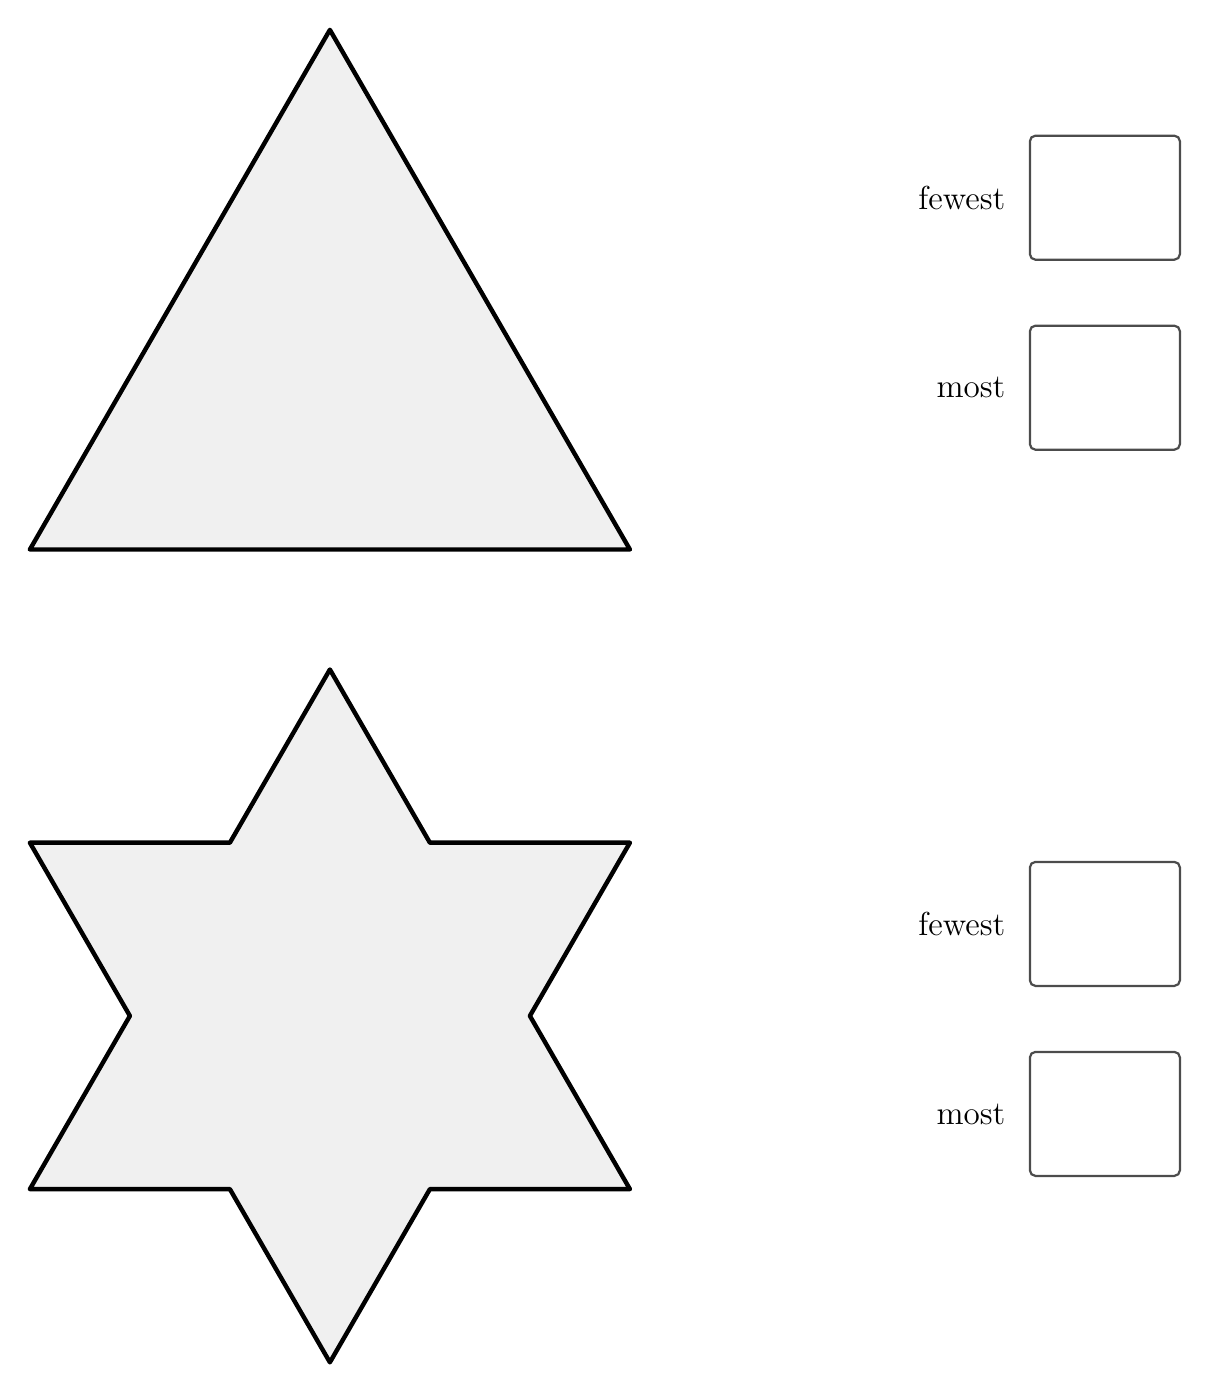
\begin{tikzpicture}[x=1in,y=1in]
\fill[black!6, even odd rule] (2,2.5981) -- (1,2.5981) -- (1.5,1.7321) -- (1,0.866) -- (2,0.866) -- (2.5,0) -- (3,0.866) -- (4,0.866) -- (3.5,1.7321) -- (4,2.5981) -- (3,2.5981) -- (2.5,3.4641) -- cycle;
\draw[line width=1.6pt, black, line join=round] (2,2.5981) -- (1,2.5981) -- (1.5,1.7321) -- (1,0.866) -- (2,0.866) -- (2.5,0) -- (3,0.866) -- (4,0.866) -- (3.5,1.7321) -- (4,2.5981) -- (3,2.5981) -- (2.5,3.4641) -- cycle;
\node[anchor=east, inner sep=0pt] at (5.88,1.2421) {\large most};
\draw[line width=0.8pt, black!70, rounded corners=2pt] (6,0.9321) rectangle (6.75,1.5521);
\node[anchor=east, inner sep=0pt] at (5.88,2.1921) {\large fewest};
\draw[line width=0.8pt, black!70, rounded corners=2pt] (6,1.8821) rectangle (6.75,2.5021);
\fill[black!6, even odd rule] (4,4.0641) -- (2.5,6.6622) -- (1,4.0641) -- cycle;
\draw[line width=1.6pt, black, line join=round] (4,4.0641) -- (2.5,6.6622) -- (1,4.0641) -- cycle;
\node[anchor=east, inner sep=0pt] at (5.88,4.8731) {\large most};
\draw[line width=0.8pt, black!70, rounded corners=2pt] (6,4.5631) rectangle (6.75,5.1831);
\node[anchor=east, inner sep=0pt] at (5.88,5.8231) {\large fewest};
\draw[line width=0.8pt, black!70, rounded corners=2pt] (6,5.5131) rectangle (6.75,6.1331);
\end{tikzpicture}
